% Compile:  cd paper && tectonic main.tex
% Every number comes from paper/tables/*.tex, written by src/report.py and src/fertility.py
% from the saved model outputs in results/. Rerunning them regenerates the tables and figures.

\documentclass[11pt]{article}
\usepackage[review]{acl}   % [review] = anonymous submission; [preprint] = arXiv with author names
\usepackage{times}
\usepackage{latexsym}
\usepackage[T1]{fontenc}
\usepackage[utf8]{inputenc}
\usepackage{microtype}
\usepackage{inconsolata}
\usepackage{graphicx}
\usepackage{booktabs}
\usepackage{amsmath}
\usepackage{xcolor}

\newcommand{\NumEval}{200}
\newcommand{\NumSeeds}{3}
\newcommand{\EvalDevice}{Apple M1 Pro (MPS)}
\newcommand{\MaxNewTokens}{768}
\newcommand{\MaxRefTokens}{384}
\newcommand{\RefAcc}{17.5}
\newcommand{\RefSize}{4.87}
\newcommand{\ParamsTotal}{2.61}
\newcommand{\ParamsQuant}{2.02}
\newcommand{\ParamsQuantShare}{77}
\newcommand{\NumCalib}{128}

\newcommand{\AccBangla}{16.7 $\pm$ 1.2}
\newcommand{\DropBangla}{$-0.8$}
\newcommand{\AccEnglishMath}{13.8 $\pm$ 2.3}
\newcommand{\DropEnglishMath}{$-3.7$}
\newcommand{\AccEnglishWiki}{13.0 $\pm$ 0.9}
\newcommand{\DropEnglishWiki}{$-4.5$}
\newcommand{\AccBanglaParallel}{17.3 $\pm$ 0.8}
\newcommand{\DropBanglaParallel}{$-0.2$}
\newcommand{\AccEnglishParallel}{15.7 $\pm$ 3.3}
\newcommand{\DropEnglishParallel}{$-1.8$}
\newcommand{\AccRtnFour}{10.5}
\newcommand{\DropRtnFour}{$-7.0$}
\newcommand{\AccRtnThree}{0.0}
\newcommand{\DropRtnThree}{$-17.5$}
\newcommand{\AccGptqThree}{14.5}
\newcommand{\DropGptqThree}{$-3.0$}
\newcommand{\AccNfFour}{15.0}
\newcommand{\DropNfFour}{$-2.5$}
\newcommand{\AccRtnEight}{17.5}
\newcommand{\DropRtnEight}{$+0.0$}
\newcommand{\DeltaLangDomain}{$+3.7$~pp (95\% CI [+0.7, +6.8])}
\newcommand{\PLangDomain}{0.078}
\newcommand{\DeltaLang}{$+2.8$~pp (95\% CI [-0.5, +6.2])}
\newcommand{\PLang}{0.301}
\newcommand{\DeltaDomain}{$+0.8$~pp (95\% CI [-2.5, +4.0])}
\newcommand{\PDomain}{0.782}
\newcommand{\DeltaGptqRtn}{$+6.2$~pp (95\% CI [+1.7, +10.7])}
\newcommand{\PGptqRtn}{0.007}
\newcommand{\DeltaGptqRtnThree}{$+14.5$~pp (95\% CI [+10.0, +19.5])}
\newcommand{\PGptqRtnThree}{$<$0.001}
\newcommand{\DeltaLangParallel}{$+1.7$~pp (95\% CI [-2.0, +5.3])}
\newcommand{\PLangParallel}{0.782}

\newcommand{\RepDeltaLangDomain}{$-8.2$~pp (95\% CI [-13.3, -3.2])}
\newcommand{\RepPLangDomain}{0.002}
\newcommand{\RepDeltaLang}{$-9.7$~pp (95\% CI [-15.0, -4.5])}
\newcommand{\RepPLang}{0.002}
\newcommand{\RepDeltaDomain}{$+1.5$~pp (95\% CI [-3.7, +6.7])}
\newcommand{\RepPDomain}{0.575}
\newcommand{\RepDeltaLangParallel}{$-10.2$~pp (95\% CI [-15.2, -5.2])}
\newcommand{\RepPLangParallel}{$<$0.001}

\newcommand{\NoiseAcc}{17.0}
\newcommand{\NoiseLost}{3}
\newcommand{\NoiseGained}{0}
\newcommand{\NoiseIdentical}{87}

\newcommand{\FertBangla}{3.49}
\newcommand{\FertEnglish}{1.18}
\newcommand{\FertRatio}{2.9}
\newcommand{\SolutionTokens}{511}

\newcommand{\CompNumeric}{120 (60\%)}
\newcommand{\CompChoice}{43 (22\%)}
\newcommand{\CompExpression}{37 (18\%)}

\makeatletter\newcommand{\tablebody}[1]{\@@input #1 }\makeatother  % plain-TeX input works inside tabular

\title{Calibration Language Changes How Quantized Models Fail:\\A Case Study of a Small {Bangla} Math {LLM}}

\author{Ajoy Sarker \and Shreya Nag Riya \\
  Department of Computer Science and Engineering \\
  Jahangirnagar University, Dhaka, Bangladesh \\
  \texttt{\{ajoy.stu20181, nag.stu2018\}@juniv.edu}}

\begin{document}
\maketitle

% ================================================================ abstract
\begin{abstract}
% (1) context
Quantization lets large language models (LLMs) run on low-cost hardware, often the only option for speakers of languages such as Bangla.
% (2) gap
Yet quantization is calibrated almost only on English, and its effect on other languages is poorly understood, although Bangla needs \FertRatio$\times$ more tokens per word, giving quantization error more steps to accumulate.
% (3) aim
We ask how quantization, and the language of its calibration data, affect a small Bangla math model.
% (4) design
We quantize Gemma-2~2B, fine-tuned on Bangla math, with round-to-nearest (RTN), NF4 and GPTQ at 8 to 3 bits, calibrate GPTQ on five sets including the same problems in Bangla and in English, and test \NumEval{} held-out problems with corrected paired tests.
% (5) results
8-bit RTN is lossless, 3-bit RTN solves nothing, and GPTQ beats RTN at 4 and 3 bits. Calibration language does not significantly change accuracy, but English calibration raises the share of repetitive, unfinished outputs by about 10 points ($p<0.001$), even on identical problems, while changing only the domain has no effect.
% (6) contributions
Conceptually, quantization damage in a low-resource language appears as repetition rather than language drift, and accuracy alone misses it. Practically, deployments should calibrate in the target language and monitor repetition.
\end{abstract}

% ================================================================ introduction
\section{Introduction}

Bangla is spoken by more than 230 million people, most of whom have limited access to the GPUs needed to run modern LLMs. Quantization stores weights in 8, 4 or fewer bits instead of 16, which cuts memory and cost \citep{dettmers2022llmint8,frantar2023gptq}.

Quantization adds rounding error to every weight. The best methods, such as GPTQ \citep{frantar2023gptq} and AWQ \citep{lin2024awq}, reduce this error using a small \emph{calibration set} of example inputs, which in practice is usually English web text. For a model used in Bangla, this default is questionable for two reasons. First, the model's internal activations on Bangla text may differ from those on English. Second, Bangla is split into far more tokens per word than English \citep{petrov2023tokenizer,ahia2023languages}, so a solution takes more generation steps, and a small error has more chances to derail it. Step-by-step mathematics is especially exposed, because one wrong step makes the final answer wrong.

Prior work shows that quantization hurts non-Latin-script languages more than English \citep{marchisio2024quantization} and that calibration data matter for compressed models \citep{williams2024calibration,zeng2024multilingual}. We study the question in a concrete setting: one small model, fine-tuned for one task in one low-resource language. We make three contributions:

\begin{enumerate}
  \setlength\itemsep{0pt}
  \item We compare seven quantization configurations from 8 to 3 bits and show that the quantization method matters far more than the bit width alone: GPTQ keeps nearly all accuracy at 4 bits, while plain rounding collapses at 3 bits.
  \item We separate the effect of calibration \emph{language} from \emph{domain}, including a parallel design that calibrates on the same problems in Bangla and in English. Calibration language has no significant effect on accuracy but a large, significant effect on how often outputs fall into repetition loops.
  \item We show that accuracy hides much of what quantization changes: models fail by repeating themselves rather than by switching to English, and even an 8-bit model with unchanged accuracy solves a noticeably different set of problems, well beyond what numerical noise explains.
\end{enumerate}

% ================================================================ related work
\section{Related Work}

\paragraph{Post-training quantization.}
LLM.int8 \citep{dettmers2022llmint8} stores weights in 8 bits and keeps outlier features in 16 bits. NF4 \citep{dettmers2023qlora} places 16 levels according to a normal distribution and is the base format of QLoRA fine-tuning. GPTQ \citep{frantar2023gptq} quantizes weights column by column and uses calibration inputs to correct the error of each step. AWQ \citep{lin2024awq} and SmoothQuant \citep{xiao2023smoothquant} also rely on calibration activations.

\paragraph{Calibration data and languages.}
\citet{williams2024calibration} show that the choice of calibration data changes the downstream performance of quantized and pruned models. \citet{zeng2024multilingual} show that English-only calibration disadvantages other languages when compressing multilingual models. \citet{marchisio2024quantization} find that quantization harms non-Latin-script languages most and that automatic metrics underestimate the damage. We add a parallel design that holds the calibration problems fixed and changes only their language, and we measure how failures change, not only accuracy.

\paragraph{Bangla mathematical reasoning.}
English math benchmarks such as GSM8K \citep{cobbe2021gsm8k} and MATH \citep{hendrycks2021math} have Bangla counterparts only recently; BEnQA \citep{shafayat2024benqa} shows a large gap between Bangla and English reasoning even for strong models. We use a public Bangla math corpus with step-by-step solutions \citep{ashrafur2024banglamath}, which is a Bangla translation of NuminaMath-CoT \citep{numinamath2024}.

% ================================================================ setup
\section{Experimental Setup}

\paragraph{Model.}
We fine-tune Gemma-2~2B-it \citep{gemma2024gemma2} with QLoRA \citep{dettmers2023qlora,hu2022lora} on 3,000 problem--solution pairs from the Bangla dataset. LoRA (rank 16, $\alpha=16$) is applied to all attention and MLP projections; we train for 400 steps with effective batch size 8 and learning rate $2\times10^{-4}$. The adapter is merged into the 16-bit model, which serves as the reference and as the input to every quantization method. Of the model's \ParamsTotal{}B parameters, \ParamsQuant{}B (\ParamsQuantShare\%) are in the linear layers of the transformer blocks; only these are quantized, as is standard.

\paragraph{Quantization methods.}
\textbf{RTN} rounds each weight to the nearest of $2^b$ levels, with a scale and zero point per output row (8-bit) or per group of 128 weights (4 and 3-bit). \textbf{NF4} uses the 16 levels of \citet{dettmers2023qlora} with one scale per block of 64 weights. \textbf{GPTQ} \citep{frantar2023gptq} uses the same groups as RTN but quantizes columns in order and adjusts the remaining weights to compensate for each rounding error, using statistics from the calibration set. Comparing GPTQ with RTN at equal size therefore isolates the value of calibration.

We use \emph{simulated} quantization: weights are rounded and stored back in 16-bit, so the model computes with exactly the values a low-bit kernel would use. This is standard for measuring accuracy and lets every method run on the same machine (\EvalDevice). Sizes are computed from the bit widths; we do not report speed, which depends on hardware kernels rather than on the method.

\paragraph{Calibration sets.}
Table~\ref{tab:calib} lists the five calibration sets, each with \NumCalib{} samples of up to 512 tokens. The first three follow common practice; English Wikipedia is WikiText-2 \citep{merity2017wikitext}. The last two form a \emph{parallel} pair: we matched Bangla training problems to their English originals in NuminaMath-CoT by their numbers and final answers (1,370 unique matches), so the two sets contain exactly the same problems and differ only in language. Each 4-bit configuration is quantized with \NumSeeds{} random samples (seeds); 3-bit GPTQ uses one seed.

\begin{table}[t]
\centering
\small
\begin{tabular}{lll}
\toprule
Calibration set & Language & Content \\
\midrule
Bangla math & Bangla & training problems \\
English GSM8K & English & grade-school math \\
English Wikipedia & English & WikiText-2 text \\
\midrule
Bangla parallel & Bangla & matched problems \\
English parallel & English & same, original English \\
\bottomrule
\end{tabular}
\caption{GPTQ calibration sets. English GSM8K vs.\ English Wikipedia changes only the domain; the parallel pair changes only the language.}
\label{tab:calib}
\end{table}

\paragraph{Evaluation.}
The test set has \NumEval{} problems drawn from rows never used in training. We keep problems with an automatically checkable answer and a reference solution of at most \MaxRefTokens{} tokens, about a third of the data, so that a complete solution fits in the generation budget. The answers are numbers (\CompNumeric), multiple-choice letters (\CompChoice) or short expressions (\CompExpression). Models decode greedily for up to \MaxNewTokens{} tokens. A problem counts as solved if the last \texttt{\textbackslash boxed\{\}} answer matches the reference after normalization (Bangla digits, LaTeX formatting, units, numeric tolerance, and choice letters matched to option values).

For failed problems we record the failure type: a \emph{wrong} answer, no answer within the token \emph{limit}, or \emph{stopped} without an answer. We also mark an output as \emph{repetitive} if any sequence of eight words occurs three or more times, and as \emph{drifting} if fewer than half of its letters are Bangla script.

\paragraph{Statistics.}
All models answer the same problems, so we compare them with a paired bootstrap over problems \citep{koehn2004significance} (10,000 resamples), averaging over seeds first. We correct for multiple comparisons with the Holm method within each research question: all methods against 16-bit; GPTQ against RTN; and the calibration comparisons, separately for accuracy and repetition. To separate quantization effects from numerical noise, we run the 16-bit model a second time with a different batch size.

% ================================================================ results
\section{Results}

\begin{table*}[t]
\centering
\small
\resizebox{\textwidth}{!}{%
\begin{tabular}{lrrrrr}
\toprule
Method & Bits/weight & Size (GB) & Accuracy (\%) & $\Delta$ vs.\ 16-bit (pp) [95\% CI] & Lost / gained (\%) \\
\midrule
\tablebody{tables/main.tex}
\bottomrule
\end{tabular}}
\caption{Accuracy and size on \NumEval{} held-out Bangla math problems. 4-bit GPTQ rows are mean~$\pm$~std over \NumSeeds{} calibration seeds. $\Delta$: paired-bootstrap difference; * = significant after Holm correction over the ten comparisons with 16-bit. Lost / gained: share of problems solved by 16-bit that the quantized model fails, and share of 16-bit failures it solves.}
\label{tab:main}
\end{table*}

\subsection{The method matters more than the bit width}

Table~\ref{tab:main} summarizes accuracy and size. The 16-bit model solves \RefAcc\% of the problems.

\textbf{8 bits cost nothing.} RTN 8-bit shrinks the model from \RefSize{} to 2.99~GB (39\% smaller) with identical accuracy.

\textbf{At 4 bits, calibration-based correction helps.} Plain RTN drops to \AccRtnFour\%, while GPTQ keeps \AccBangla\% at the same size, a difference of \DeltaGptqRtn{} (Holm $p=\PGptqRtn$). NF4 lies in between.

\textbf{At 3 bits, RTN collapses.} It solves no problem at all, while 3-bit GPTQ still solves \AccGptqThree\% (difference \DeltaGptqRtnThree, $p<0.001$).

Against 16-bit, only the 3-bit RTN drop survives the Holm correction; 4-bit losses of 0.2 to 7 points are too small to confirm with \NumEval{} problems.

\begin{figure*}[t]
\centering
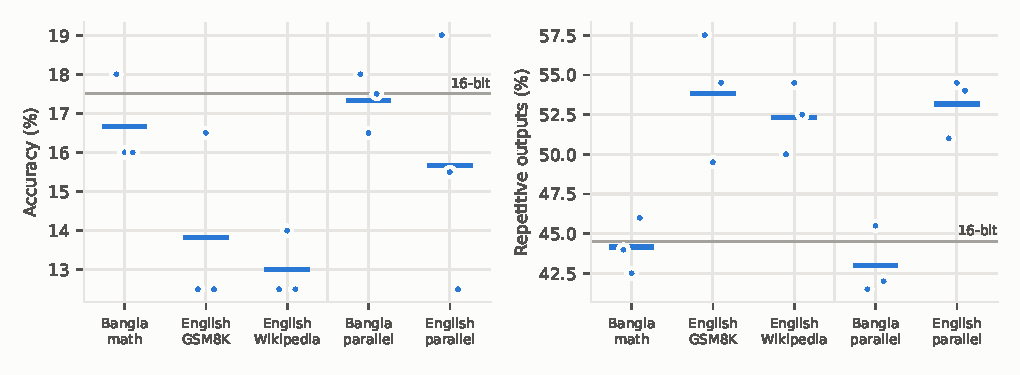
\includegraphics[width=0.82\textwidth]{../results/fig_calibration.pdf}
\caption{4-bit GPTQ under each calibration set. Left: accuracy. Right: share of outputs that fall into repetition loops. Dots are calibration seeds, bars are means, grey lines show the 16-bit model. The two rightmost sets contain the same problems in Bangla and English.}
\label{fig:calibration}
\end{figure*}

\subsection{Calibration language changes failures, not accuracy}

Figure~\ref{fig:calibration} compares the five calibration sets for 4-bit GPTQ.

\textbf{Accuracy.} Bangla calibration gives the highest accuracy in both designs: \AccBangla\% for Bangla math versus \AccEnglishWiki\% for English Wikipedia, and \AccBanglaParallel\% versus \AccEnglishParallel\% for the parallel pair. None of these differences is significant after correction (Bangla math vs.\ English Wikipedia: \DeltaLangDomain, Holm $p=\PLangDomain$; parallel pair: \DeltaLangParallel, $p=\PLangParallel$). Seed-to-seed differences are as large as differences between sets (English parallel: 12.5--19.0\%).

\textbf{Repetition.} The language of the calibration set has a clear effect on how the model fails. With Bangla calibration, 43--44\% of outputs contain a repetition loop, the same as the 16-bit model (44.5\%). With any English calibration set, 52--54\% do. On identical problems, switching the calibration language from English to Bangla reduces repetitive outputs by \RepDeltaLangParallel{} (Holm $p<0.001$). Changing only the domain, from English Wikipedia to English math, has no effect (\RepDeltaDomain, $p=\RepPDomain$). The cause is the calibration language, not the topic.

\subsection{Quantized models repeat; they do not drift}

\begin{table}[t]
\centering
\small
\setlength{\tabcolsep}{3pt}
\resizebox{\columnwidth}{!}{%
\begin{tabular}{lrrrrrr}
\toprule
Method & Wrong & Limit & Stopped & Repet. & Drift & Tokens \\
\midrule
\tablebody{tables/errors.tex}
\bottomrule
\end{tabular}}
\caption{Failure types, \% of problems. \emph{Wrong}: incorrect boxed answer. \emph{Limit}: no answer within \MaxNewTokens{} tokens. \emph{Stopped}: ended without an answer. \emph{Repet.}: output contains a repetition loop. \emph{Drift}: mostly non-Bangla output. \emph{Tokens}: mean output length.}
\label{tab:errors}
\end{table}

Table~\ref{tab:errors} shows how models fail. Even the 16-bit model fails in two main ways: a wrong answer (39.5\%) or no answer within the token limit (39.5\%). The second kind is almost always a loop: 82--99\% of outputs that hit the limit are repetitive, in every configuration.

Quantization error shifts failures toward these loops. Unfinished outputs rise from 39.5\% (16-bit) to 52.5\% with RTN 4-bit and 98.5\% with RTN 3-bit, and outputs grow longer (from 499 to 565 and 761 tokens on average). A typical RTN 3-bit output ends by repeating, in Bangla, ``\dots to consider how many possible cases of the divisor there are, based on the relation between dividend and remainder, we\dots'' until the budget runs out.

Language drift, by contrast, is negligible: at most 0.5\% of outputs are mostly non-Bangla in any configuration, including the English-calibrated ones. English calibration damages the coherence of long Bangla generations, not the choice of language.

\subsection{Equal accuracy hides different answers}

The last column of Table~\ref{tab:main} shows that quantized models solve different problems, not just fewer. RTN 8-bit has the same accuracy as 16-bit, yet it fails 23\% of the problems the 16-bit model solved and solves 5\% of those it failed; for 4-bit GPTQ with Bangla calibration the figures are 45\% and 8\%. This churn is not numerical noise: rerunning the 16-bit model with a different batch size reproduces \NoiseIdentical\% of outputs exactly and changes only \NoiseLost\% of solved problems.

\subsection{Why long outputs matter for Bangla}

Gemma's tokenizer uses \FertBangla{} tokens per word on Bangla solutions and \FertEnglish{} on English text (\FertRatio$\times$); the median reference solution is \SolutionTokens{} tokens long. Each generation step is a chance for quantization error to start a loop, consistent with damage appearing mainly as unfinished, repetitive output.

% ================================================================ conclusion
\section{Conclusion}

For a small Bangla math model, the quantization method matters more than the bit width, and the calibration language changes how the model fails rather than how often it succeeds: English calibration makes outputs fall into repetition loops about ten points more often, even on identical problems. For low-resource deployments, we recommend calibrating in the target language, comparing several calibration seeds, and monitoring repetition and unfinished answers, which accuracy and language-identification checks both miss.

% ================================================================ limitations
\section*{Limitations}

We study one model (Gemma-2~2B) fine-tuned on one machine-translated dataset, so results may not transfer to larger models, other languages or other tasks. The test set contains \NumEval{} problems with the shortest third of reference solutions; with this sample, accuracy differences of a few points cannot be confirmed, and 3-bit GPTQ was run with a single seed. The repetition measure was defined after we observed that most unfinished outputs were loops, so the repetition comparisons are a secondary analysis, although they are corrected for multiple testing. One of the 24 GPTQ runs was interrupted by memory pressure and resumed after re-quantizing with the same seed and calibration data; we did not verify that the two quantizations are bit-identical. We use simulated quantization, which reproduces accuracy but not speed, and does not model LLM.int8's outlier handling or NF4's double quantization. Answer matching is automatic and ignores the quality of the reasoning and the Bangla prose. We do not study activation quantization, AWQ, or 2-bit weights.

% ================================================================ ethics
\section*{Ethical Considerations}

The model is a study object, not a tutoring system: even before quantization it solves only \RefAcc\% of the test problems and can produce fluent but wrong solutions. All data are public and contain no personal information.

\section*{Acknowledgments}

We used an AI assistant (Claude, Anthropic) for help with code and for editing the text. The authors checked all code, results and text and take full responsibility for them.

\bibliography{references}

\end{document}
